\documentclass[aspectratio=169,xcolor={dvipsnames}]{beamer}

% XeLaTeX packages
\usepackage{fontspec}
\usepackage{xcolor}
\usepackage{tikz}
\usetikzlibrary{positioning}
\usepackage{booktabs}
\usepackage{amsmath}
\usepackage{amsthm}
\usepackage{caption}
\usepackage{graphicx}
\usepackage{listings}
\usepackage{biblatex}

% Bibliography
\addbibresource{references_new.bib}

% Modern theme configuration
\usetheme{Boadilla}
\usecolortheme{default}

% Define complementary palette based on VU Blue
\definecolor{VUBlue}{HTML}{0057B7}
\definecolor{Endeavour}{HTML}{0754AA}
\definecolor{AbsoluteZero}{HTML}{055AB9}
\definecolor{ScienceBlue}{HTML}{0360C8}
\definecolor{RustyNail}{HTML}{8E4F09}
\definecolor{RichGold}{HTML}{9C5608}
\definecolor{LightGray}{HTML}{F8F9FA}
\definecolor{Charcoal}{HTML}{222831}

% Set theme colors
\setbeamercolor{frametitle}{bg=VUBlue, fg=white}
\setbeamercolor{title}{fg=VUBlue}
\setbeamercolor{structure}{fg=ScienceBlue}
\setbeamercolor{alerted text}{fg=RustyNail}
\setbeamercolor{block title}{bg=AbsoluteZero, fg=white}
\setbeamercolor{block body}{bg=LightGray, fg=Charcoal}

% Font settings
\setmainfont{Liberation Sans}
\setsansfont{Liberation Sans}
\setmonofont{Liberation Mono}[Scale=0.9]

% Custom commands
\newcommand{\highlight}[1]{\textcolor{RustyNail}{\textbf{#1}}}
\newcommand{\code}[1]{\texttt{\small #1}}
\newcommand{\phase}[1]{\textcolor{ScienceBlue}{\textbf{Phase #1}}}

% Configure listings
\lstset{
  basicstyle=\ttfamily\footnotesize,
  backgroundcolor=\color{LightGray},
  frame=single,
  breaklines=true
}

% Title page info
\title{Privacy-Preserving Synthetic Trajectory Generation}
\subtitle{An Integrated DiffTraj-LM-TAD Framework for Taxi Route Anomaly Detection}
\author{Mateusz Kędzia}
\institute{MSc Artificial Intelligence \\ Vrije Universiteit Amsterdam}
\date{Thesis Progress Presentation -- July 2025}

% Custom title page
\defbeamertemplate*{title page}{customized}[1][]
{%
  \vbox{}
  \vfill
  \begingroup
    \centering
    \begin{beamercolorbox}[sep=8pt,center,#1]{title}
      \usebeamerfont{title}\inserttitle\par%
      \ifx\insertsubtitle\@empty%
      \else%
        \vskip0.25em%
        {\usebeamerfont{subtitle}\usebeamercolor[fg]{subtitle}\insertsubtitle\par}%
      \fi%     
    \end{beamercolorbox}%
    \vskip1em\par
    \begin{beamercolorbox}[sep=8pt,center,#1]{author}
      \usebeamerfont{author}\insertauthor
    \end{beamercolorbox}
    \begin{beamercolorbox}[sep=8pt,center,#1]{institute}
      \usebeamerfont{institute}\insertinstitute
    \end{beamercolorbox}
    \begin{beamercolorbox}[sep=8pt,center,#1]{date}
      \usebeamerfont{date}\insertdate
    \end{beamercolorbox}\vskip0.5em
  \endgroup
  \vfill
}

\begin{document}

% --- Redesigned Title Slide ---
\begin{frame}[plain]
  \vspace{1.5cm}
  \centering
  {\usebeamerfont{title}\color{VUBlue}\Huge\textbf{Privacy-Preserving Synthetic Trajectory Generation}}
  
  \vspace{0.5em}
  {\usebeamerfont{subtitle}\color{RichGold}\Large An Integrated DiffTraj-LM-TAD Framework}
  
  \vspace{1.5em}
  {\usebeamerfont{author}\large Mateusz Kędzia}
  
  \vspace{0.5em}
  {\usebeamerfont{institute}\normalsize MSc Artificial Intelligence \\ Vrije Universiteit Amsterdam}
  
  \vspace{1em}
  {\usebeamerfont{date}\small Thesis Progress Presentation -- July 2025}
\end{frame}

% --- Redesigned Core Challenge Slide ---
\begin{frame}{The Core Challenge}
  \begin{columns}[T,onlytextwidth]
    \begin{column}{0.6\textwidth}
      \begin{alertblock}{Privacy vs. Utility}
        \vspace{0.5em}
        \highlight{High Utility}: Trajectory data = valuable insights \\
        \highlight{High Risk}: Location patterns = privacy threat \\
        \vspace{0.5em}
        \textcolor{Charcoal}{\small Standard privacy methods degrade spatio-temporal patterns}
      \end{alertblock}
    \end{column}
    \begin{column}{0.4\textwidth}
      \centering
      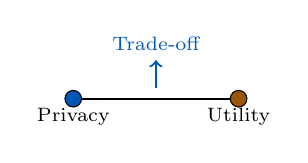
\begin{tikzpicture}[scale=0.7]
        % Privacy vs Utility scale
        \draw[thick] (0,0) -- (3,0);
        \draw[fill=VUBlue] (0,0) circle (0.15);
        \draw[fill=RichGold] (3,0) circle (0.15);
        \node[below] at (0,0) {\scriptsize Privacy};
        \node[below] at (3,0) {\scriptsize Utility};
        \draw[thick,->,VUBlue] (1.5,0.2) -- (1.5,0.7);
        \node[above,VUBlue] at (1.5,0.7) {\scriptsize Trade-off};
      \end{tikzpicture}
    \end{column}
  \end{columns}
\end{frame}

% --- Redesigned Research Gap Slide ---
\begin{frame}{Research Gap}
  \begin{columns}[T,onlytextwidth]
    \begin{column}{0.48\textwidth}
      \begin{block}{Key Problems}
        \begin{itemize}
          \item \highlight{Data Scarcity}
          \item \highlight{Privacy Barriers}
          \item \highlight{Detection Limitations}
        \end{itemize}
      \end{block}
    \end{column}
    \hspace{0.04\textwidth}
    \begin{column}{0.48\textwidth}
      \begin{block}{Our Innovation}
        \centering
        \textbf{Privacy by Design} $\rightarrow$ \textbf{High Utility} $\rightarrow$ \textbf{Anomaly Detection Ready}
      \end{block}
    \end{column}
  \end{columns}
\end{frame}

% --- Redesigned Solution Slide with Diagram ---
\begin{frame}{The Solution: 3-Phase Framework}
  \begin{block}{Framework Overview}
    \centering
    \phase{1}: Baseline $\rightarrow$ \phase{2}: Anomaly Mining $\rightarrow$ \phase{3}: Enhanced Model
  \end{block}
  \vspace{1em}
  \begin{center}
    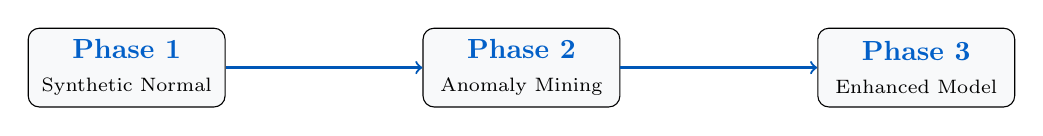
\begin{tikzpicture}[node distance=2.5cm, every node/.style={align=center}]
      % Nodes
      \node[draw, fill=LightGray, rounded corners, minimum width=2.5cm, minimum height=1cm] (phase1) {\phase{1}\\\scriptsize Synthetic Normal};
      \node[draw, fill=LightGray, rounded corners, right=of phase1, minimum width=2.5cm, minimum height=1cm] (phase2) {\phase{2}\\\scriptsize Anomaly Mining};
      \node[draw, fill=LightGray, rounded corners, right=of phase2, minimum width=2.5cm, minimum height=1cm] (phase3) {\phase{3}\\\scriptsize Enhanced Model};
      % Arrows
      \draw[thick, VUBlue,->] (phase1) -- (phase2);
      \draw[thick, VUBlue,->] (phase2) -- (phase3);
    \end{tikzpicture}
  \end{center}
  \vspace{1em}
  \begin{columns}[T,onlytextwidth]
    \begin{column}{0.33\textwidth}
      \centering\scriptsize Real Data $\rightarrow$ DiffTraj
    \end{column}
    \begin{column}{0.33\textwidth}
      \centering\scriptsize LM-TAD $+$ Curation
    \end{column}
    \begin{column}{0.33\textwidth}
      \centering\scriptsize Retrain $+$ Refine
    \end{column}
  \end{columns}
\end{frame}

\begin{frame}{Key Innovation: Bootstrap Approach}
  \begin{alertblock}{Bootstrap Methodology}
    \centering
    \large\textit{``Bootstraps anomaly generation without pre-labeled dataset''}
  \end{alertblock}
  
  \vspace{1em}
  \begin{block}{Why This Works}
    \begin{itemize}
      \item \textbf{Iterative Learning}: Each cycle improves understanding
      \item \textbf{Controlled Generation}: Rule-based curation
      \item \textbf{Privacy First}: From distributions, not copies
    \end{itemize}
  \end{block}
\end{frame}

\begin{frame}{Core Model 1: DiffTraj \cite{zhuDiffTrajGeneratingGPS2023}}
  \begin{block}{Diffusion-Based Generation}
    \centering
    \textit{``Diffusion Probabilistic Model for GPS Trajectory Generation''}
  \end{block}
  
  \vspace{1em}
  \begin{columns}
    \begin{column}{0.6\textwidth}
      \begin{block}{Key Process}
        \centering
        \textbf{White Noise} $\rightarrow$ \textbf{Reverse Denoising} $\rightarrow$ \textbf{Realistic Trajectory}
      \end{block}
    \end{column}
    \begin{column}{0.4\textwidth}
      \begin{block}{Architecture}
        \begin{itemize}
          \item 1D-CNN-based residual network with attention
          \item Works directly with continuous GPS coordinates
        \end{itemize}
      \end{block}
    \end{column}
  \end{columns}
\end{frame}

\begin{frame}{Why DiffTraj?}
  \begin{table}[h]
    \centering
    \begin{tabular}{lccc}
      \toprule
      \textbf{Feature} & \textbf{DiffTraj} & \textbf{GANs} & \textbf{VAEs} \\
      \midrule
      Training Stability & \highlight{Excellent} & Mode collapse & Good \\
      Sample Quality & \highlight{High-fidelity} & Good & Blurry \\
      Privacy Protection & \highlight{Inherent} & Risk & Risk \\
      Controllability & \highlight{Conditional} & Limited & Good \\
      \bottomrule
    \end{tabular}
  \end{table}
\end{frame}

\begin{frame}{Core Model 2: LM-TAD \cite{mbuyaTrajectoryAnomalyDetection2024}}
  \begin{block}{Language Model for Trajectories}
    \centering
    \textit{``Treats trajectories as sequences of tokens''}
  \end{block}
  
  \vspace{1em}
  \begin{columns}
    \begin{column}{0.6\textwidth}
      \begin{block}{Process}
        \centering
        \textbf{GPS Trajectory} $\rightarrow$ \textbf{Token Sequence} $\rightarrow$ \textbf{Transformer} $\rightarrow$ \textbf{Perplexity Score}
      \end{block}
    \end{column}
    \begin{column}{0.4\textwidth}
      \begin{block}{Key Features}
        \begin{itemize}
          \item \textbf{Autoregressive}: Predicts next location
          \item \textbf{Perplexity Scoring}: Higher = more anomalous
          \item \textbf{Interpretable}: Clear anomaly explanations
        \end{itemize}
      \end{block}
    \end{column}
  \end{columns}
\end{frame}

\begin{frame}{Why LM-TAD?}
  \begin{columns}
    \begin{column}{0.5\textwidth}
      \begin{block}{Perfect for Bootstrapping}
        \begin{itemize}
          \item \textbf{No Labeled Data Required}
          \item \textbf{Interpretable Scores}
          \item \textbf{Online Detection Capability}
          \item \textbf{GPS Compatible}
        \end{itemize}
      \end{block}
    \end{column}
    \begin{column}{0.5\textwidth}
      \begin{alertblock}{State-of-the-Art Performance}
        \begin{itemize}
          \item Demonstrated on synthetic and real-world datasets
          \item User-specific anomaly detection
          \item Efficient attention caching
        \end{itemize}
      \end{alertblock}
    \end{column}
  \end{columns}
\end{frame}

\begin{frame}{Privacy by Design \cite{buchholzSystematisationKnowledgeTrajectory2024}}
  \begin{alertblock}{The Challenge}
    \centering
    \textit{``Traditional privacy methods destroy spatio-temporal relationships''}
  \end{alertblock}
  
  \vspace{1em}
  \begin{block}{Our Three-Layer Defense}
    \begin{enumerate}
      \item \textbf{Differential Privacy}: DP-SGD with privacy budgets
      \item \textbf{Trajectory-Level Protection}: Entire trajectory as unit
      \item \textbf{Synthetic Decoupling}: Generation from distributions
    \end{enumerate}
  \end{block}
\end{frame}

\begin{frame}{Layer 1: Differential Privacy}
  \begin{columns}
    \begin{column}{0.5\textwidth}
      \begin{block}{DP-SGD Integration}
        \begin{itemize}
          \item \textbf{Privacy Budgets}: $\varepsilon_1=2.0$, $\varepsilon_2=1.0$, $\varepsilon_3=0.5$
          \item \textbf{Bounded Influence}: Individual trajectory impact limited
          \item \textbf{Source}: PATE-GAN principles
        \end{itemize}
      \end{block}
    \end{column}
    \begin{column}{0.5\textwidth}
      \begin{block}{Protection Mechanism}
        \begin{itemize}
          \item Noise addition during training
          \item Prevents membership inference attacks
        \end{itemize}
      \end{block}
    \end{column}
  \end{columns}
\end{frame}

\begin{frame}{Phase 1: Baseline Generation}
  \begin{block}{Building the Foundation}
    \centering
    \textbf{Real Normal Data} $\rightarrow$ \textbf{Train DiffTraj} $\rightarrow$ \textbf{Synthetic Normal Data}
  \end{block}
  
  \vspace{1em}
  \begin{block}{Smart Filtering}
    \begin{itemize}
      \item \textbf{Duration}: Within $2\sigma$ of O-D medians
      \item \textbf{Distance}: $\leq 1.5 \times$ shortest path
      \item \textbf{Temporal}: Typical patterns only
    \end{itemize}
  \end{block}
\end{frame}

\begin{frame}{Phase 2: Anomaly Mining}
  \begin{block}{Unsupervised Detection Process}
    \centering
    \code{synthetic\_normal} $\rightarrow$ \textbf{LM-TAD} $\rightarrow$ \textbf{Perplexity Scoring}
  \end{block}
  
  \vspace{1em}
  \begin{columns}
    \begin{column}{0.5\textwidth}
      \begin{block}{Step 1: LM-TAD Scoring}
        \begin{itemize}
          \item \textbf{Input}: \code{synthetic\_normal} trajectories
          \item \textbf{Process}: Autoregressive language modeling
          \item \textbf{Output}: Perplexity scores (higher = more anomalous)
        \end{itemize}
      \end{block}
    \end{column}
    \begin{column}{0.5\textwidth}
      \begin{block}{Step 2: Rule-Based Curation}
        \begin{itemize}
          \item \textbf{Route Deviation}: Length $>$ Normal $+ L_\rho$
          \item \textbf{Temporal Delay}: Time $>$ Normal $+ T_\rho$
          \item \textbf{Kinematic}: Speed $> 120$ km/h
        \end{itemize}
      \end{block}
    \end{column}
  \end{columns}
\end{frame}

\begin{frame}{Phase 3: Iterative Refinement}
  \begin{block}{Closing the Loop}
    \centering
    \textbf{Normal + Anomalies} $\rightarrow$ \textbf{Retrain DiffTraj} $\rightarrow$ \textbf{Enhanced Model}
  \end{block}
  
  \vspace{1em}
  \begin{block}{Process Components}
    \begin{itemize}
      \item \textbf{Enriched Training}: 5-10\% anomalies
      \item \textbf{Iterative Cycles}: Generate $\rightarrow$ Mine $\rightarrow$ Refine
      \item \textbf{Conditional Generation}: \code{difftraj.sample(condition="speeding")}
    \end{itemize}
  \end{block}
\end{frame}

\begin{frame}{Experimental Design}
  \begin{block}{Cross-City Validation}
    \begin{table}[h]
      \centering
      \begin{tabular}{lll}
        \toprule
        \textbf{Dataset} & \textbf{Role} & \textbf{Purpose} \\
        \midrule
        \textbf{Beijing} & Primary & Framework development \\
        \textbf{Chengdu} & Validation & Cross-city generalization \\
        \textbf{Xi'an} & Validation & Urban diversity testing \\
        \bottomrule
      \end{tabular}
    \end{table}
  \end{block}
\end{frame}

\begin{frame}{Evaluation Framework}
  \begin{block}{Three-Dimensional Assessment}
    \begin{enumerate}
      \item \textbf{Anomaly Detection Performance}
      \begin{itemize}
        \item Precision, Recall, F1, AUC-PR
      \end{itemize}
      
      \item \textbf{Data Quality Assessment}
      \begin{itemize}
        \item SDMetrics (Resemblance, Utility, Privacy)
      \end{itemize}
      
      \item \textbf{Privacy Protection}
      \begin{itemize}
        \item Membership inference attacks
        \item Reconstruction attacks
      \end{itemize}
    \end{enumerate}
  \end{block}
\end{frame}

\begin{frame}{Key Contributions}
  \begin{columns}
    \begin{column}{0.5\textwidth}
      \begin{block}{Technical Innovations}
        \begin{enumerate}
          \item \textbf{Integrated Framework}: First DiffTraj + LM-TAD combination
          \item \textbf{Bootstrap Methodology}: Anomaly generation without labels
          \item \textbf{Multi-Layer Privacy}: Comprehensive protection strategy
        \end{enumerate}
      \end{block}
    \end{column}
    \begin{column}{0.5\textwidth}
      \begin{block}{Research Impact}
        \begin{itemize}
          \item Novel privacy-preserving trajectory research
          \item Reproducible evaluation framework
          \item Open-source implementation
        \end{itemize}
      \end{block}
    \end{column}
  \end{columns}
\end{frame}

\begin{frame}{Project Timeline}
  \begin{block}{Implementation Progress}
    \begin{itemize}
      \item \phase{1}: \textcolor{AbsoluteZero}{\textbf{In Progress}} (baseline DiffTraj)
      \item \phase{2}: \textbf{Planned} (LM-TAD integration)
      \item \phase{3}: \textbf{Planned} (iterative refinement)
    \end{itemize}
  \end{block}
  
  \vspace{1em}
  \begin{block}{Next Steps}
    \begin{enumerate}
      \item Complete Phase 1 baseline
      \item Implement LM-TAD integration
      \item Develop rule-based curation
      \item Cross-city validation
    \end{enumerate}
  \end{block}
\end{frame}

\begin{frame}{Expected Outcomes}
  \begin{block}{Deliverables}
    \begin{itemize}
      \item \textbf{Synthetic Datasets}: Privacy-preserving anomaly data
      \item \textbf{Open Framework}: Reproducible research pipeline
      \item \textbf{Evaluation Results}: Comprehensive performance analysis
      \item \textbf{Research Publication}: Novel methodology contribution
    \end{itemize}
  \end{block}
\end{frame}

\begin{frame}[plain]
  \centering
  \Huge \textbf{Thank You}
  
  \vspace{0.5em}
  \Large \textbf{Questions \& Discussion}
  
  \vspace{1em}
  \begin{columns}
    \begin{column}{0.5\textwidth}
      \begin{block}{Key Takeaways}
        \begin{itemize}
          \item \textbf{Privacy-Preserving}: Multi-layer protection
          \item \textbf{Bootstrap Approach}: No labeled data required
        \end{itemize}
      \end{block}
    \end{column}
    \begin{column}{0.5\textwidth}
      \begin{block}{}
        \begin{itemize}
          \item \textbf{Practical Framework}: Real-world applications
          \item \textbf{Open Research}: Reproducible and extensible
        \end{itemize}
      \end{block}
    \end{column}
  \end{columns}
\end{frame}

\begin{frame}[allowframebreaks]{References}
  \printbibliography
\end{frame}

\end{document} 